\documentclass[a4paper, 12pt]{article}

% Paquetes básicos para idioma y codificación
\usepackage[utf8]{inputenc}
\usepackage[T1]{fontenc}
\usepackage[spanish]{babel}

% Paquete para insertar imágenes
\usepackage{graphicx}

% --- PAQUETE NUEVO PARA FORZAR LA POSICIÓN DE LAS IMÁGENES ---
\usepackage{float} 

% Paquete para que el índice tenga enlaces clickeables
\usepackage[colorlinks=true, linkcolor=black, urlcolor=blue]{hyperref}

% Configuración del título
\title{Memoria de Prácticas: Ingeniería de Servidores}
\author{Juan Reche Aguilar}
\date{\today}

\begin{document}

% Genera la portada con el título
\maketitle
\clearpage % Usamos clearpage en lugar de newpage

\section{Ejercicio 4.1: Instalación y configuración de un servidor de HTTP}

En este ejercicio se decidio usar Apache como servidor web
% Imagen 1
\begin{figure}[H]
    \centering
    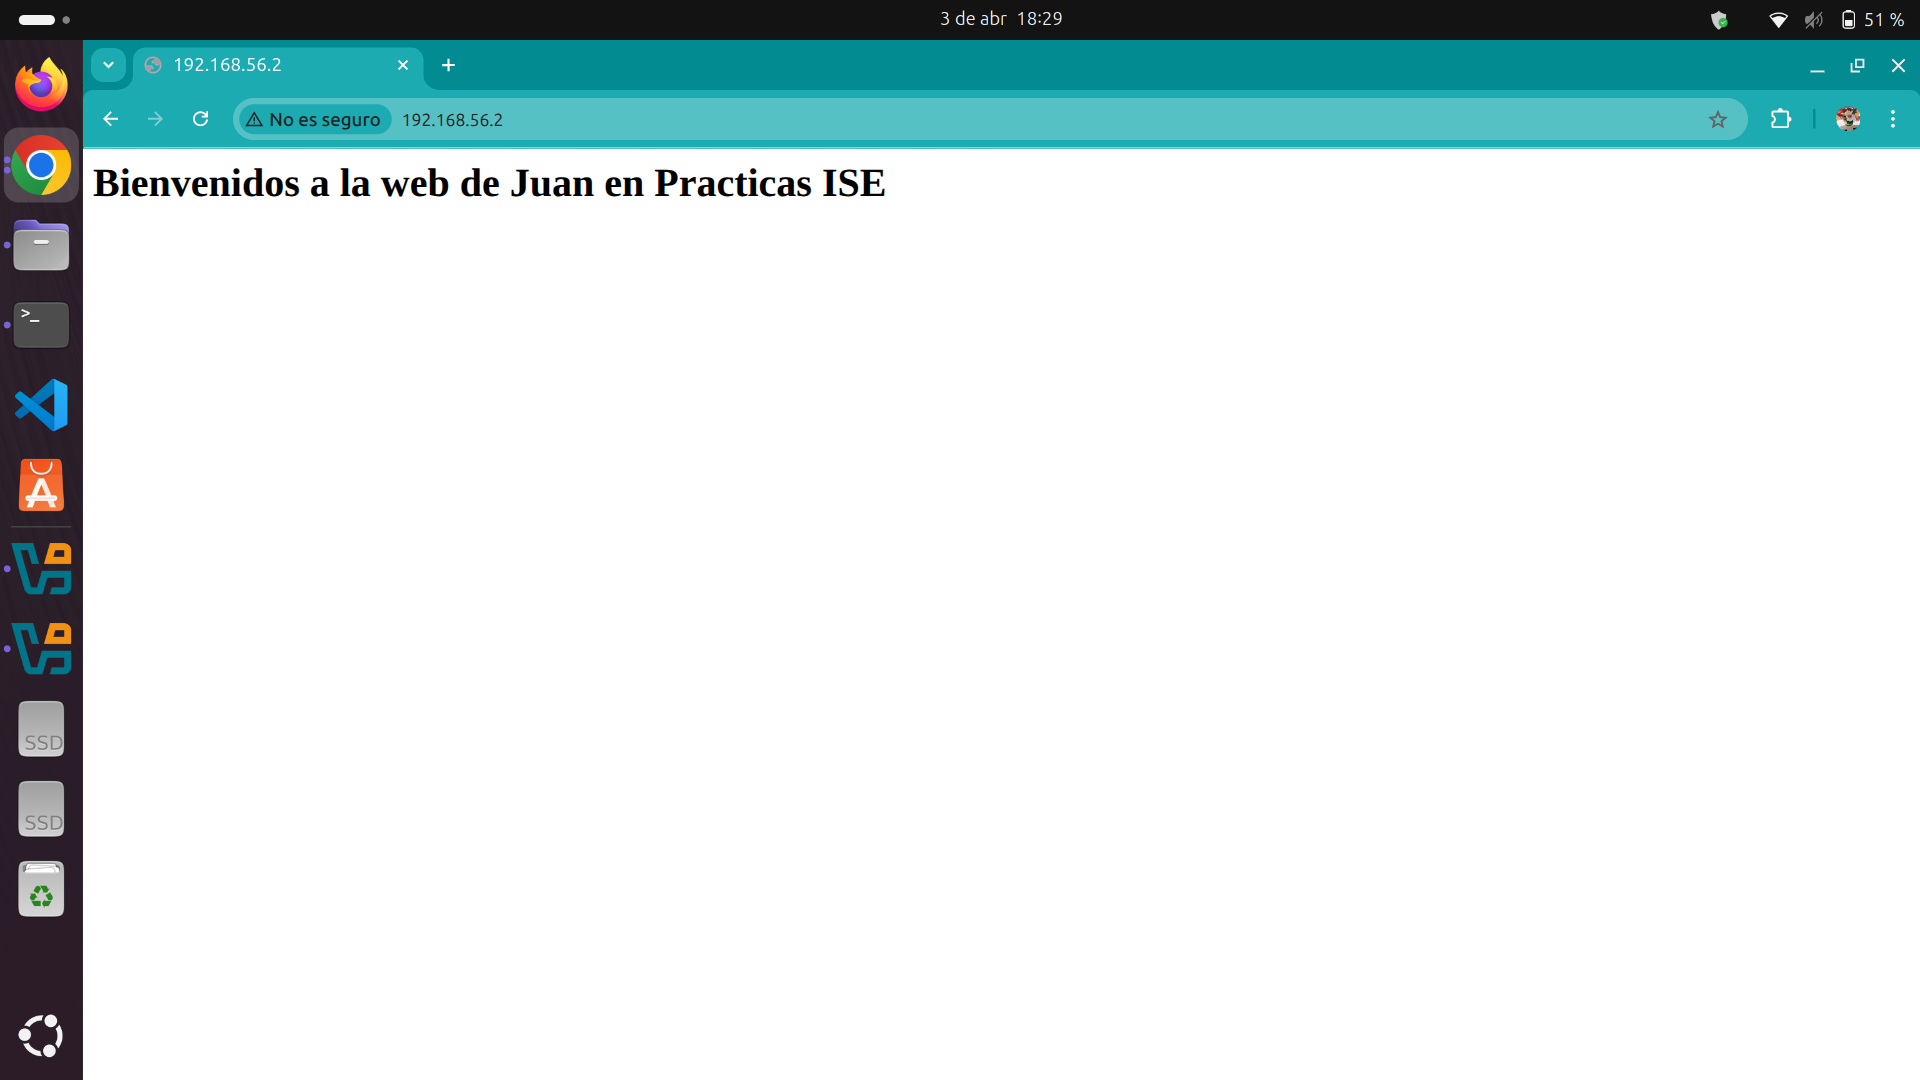
\includegraphics[width=0.8\textwidth]{../ej4/ej4_1.png}
    \caption{ Acceso desde el ordenador anfitrión, con google chrome, a la página web alojada en el servidor. 
    Se puede ver la dirección IP del servidor en la barra de direcciones.}
\end{figure}

% Imagen 2
\begin{figure}[H]
    \centering
    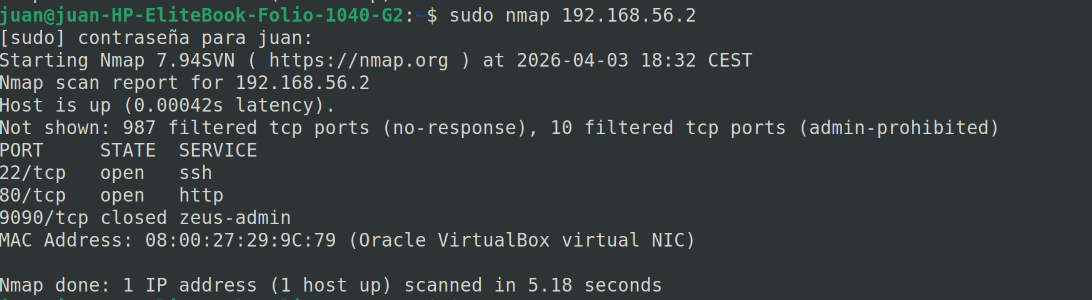
\includegraphics[width=0.8\textwidth]{../ej4/ej4_2.png}
    \caption{Resultado del comando nmap desde el ordenador anfitrión, mostrando el puerto 80 abierto en la dirección IP del servidor.}
\end{figure}

\section{Ejercicio 4.2: Configuración de SSHD}
% Imagen 3
\begin{figure}[H]
    \centering
    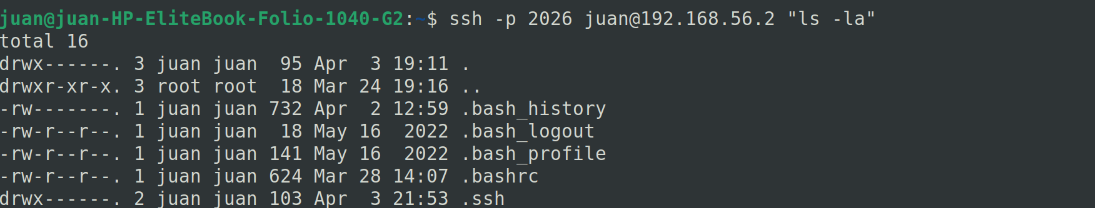
\includegraphics[width=0.8\textwidth]{../ej4/ej4_3.png}
    \caption{comando mediante ssh}
\end{figure}

% Imagen 4
\begin{figure}[H]
    \centering
    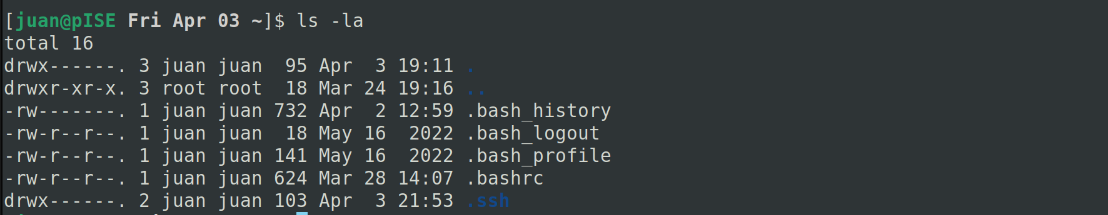
\includegraphics[width=0.8\textwidth]{../ej4/ej4_4.png}
    \caption{comando desde la terminal de la maquina virtual}
\end{figure}

Podemos ver que el resultado de ambos comando es el mismo, 
lo que indica que la conexión SSH se ha establecido correctamente y que el servidor SSH está funcionando en la máquina virtual.

\end{document}
